\chapter{Background}\label{background}

In questo Capitolo andr\`o a fare una panoramica generale di tutte le conoscenze necessarie per poter analizzare il lavoro della Tesi, spiegando cos'\`e un terremoto e tutti i termini tecnici che circondano questo campo di studio; continuer\`o dando un'introduzione alle attuali tecniche che si usano per fare previsione e presenter\`o i due algoritmi sviluppati a cavallo degli anni '80 e 90', gli algoritmi \textit{M8} e \textit{CN}. Successivamente spiegher\`o l'idea che voglio utilizzare per approcciare alla manipolazione dei dati, ovvero la Big Data Analytics, presentando qualche esempio passato alla storia che ha valorizzato questa disciplina, nata e cresciuta di pari passo con lo sviluppo di internet. La raccolta dei dati ha uno scopo essenziale, perch\'e molti dati non presentano immediatamente un'utilit\`a, ma questa potr\`a apparire con il passare del tempo, quindi raccogliere dati relativi un argomento specifico potrebbe aiutare a risolvere un problema completamente diverso in futuro. Infine andr\`o a spiegare la Formula che ho utilizzato per fare previsione nel mio lavoro, Formula ricavata dal Teorema della disuguaglianza di Chebyshev.

\section{Terremoto}\label{terremoto}
Un terremoto, detto anche \textbf{sisma} o \textbf{scossa tellurica}, \`e una vibrazione provocata quando masse di roccia che applicano una forza l'una contro l'altra, improvvisamente si fratturano.\\
La branca della geofisica che studia questi fenomeni \`e la \textbf{sismologia}.

\subsection{Onde Sismiche}

Le onde sismiche sono potenti oscillazioni, provocate dalla frattura delle rocce (vedi Sezione \ref{terremoto}). Queste vengono registrate dagli strumenti, e sono soggette ad analisi successive.\\
Le onde sismiche si dividono in due tipi, le \textbf{onde P}, sono le prime ad essere registrate dai \textbf{sismografi}\footnote{Strumenti per la misura e registrazione del moto del suolo, dotati di un sensore in grado di rilevare il passaggio delle onde sismiche generate da sorgenti di origine naturale o dall'attivit\`a dell'uomo.}, o dai \textbf{sismometri}\footnote{Strumenti che si differenziano dai sismografi, solo perch\'e effettuano la misura e non la registrazione del moto del suolo}, in quanto viaggiano quasi al doppio della velocit\`a dell'altro tipo, ovvero le \textbf{onde S}.\\
La differenza tra le due, oltre la velocit\`a di propagazione, \`e il modo in cui fanno vibrare il suolo. Il primo tipo, le onde P, lo fa nella direzione di propagazione, mentre il secondo tipo, le onde S, lo fa perpendicolarmente alla direzione di propagazione.\\
Il punto preciso dove le onde sismiche hanno avuto origine \`e chiamato \textbf{ipocentro}, ed \`e identificato da latitudine, longitudine e profondit\`a, mentre la sua proiezione verticale sulla superficie terrestre \`e chiamata \textbf{epicentro}, ed \`e il punto dove si verificano danni maggiori.\\

\subsection{Magnitudo}

Per misurare la grandezza di un terremoto abbiamo bisogno di un'unit\`a di misura, la \textbf{magnitudo}. Questa ci permette di renderci conto di quanta energia viene sprigionata dal terremoto. L'aumentare della magnitudo rappresenta un aumento non lineare dell'energia, o meglio, ogni qual volta la magnitudo aumenta di una unit\`a, l'energia sprigionata dal terremoto \`e circa 30 volte superiore.\\
La magnitudo viene misurata in vari modi, uno di questi \`e l'utilizzo di \textbf{sismogrammi}\footnote{Diagrammi tracciati dalle registrazioni fatte dai sismografi, che possono rappresentare lo spostamento, la velocit\`a o l'accelerazione del suolo in funzione del tempo}. Questo comporta che per avere una misura esatta, si devono confrontare vari dati. Vista l'urgenza da parte di Protezione Civile e Vigili del Fuoco, che devono intervenire in caso di terremoto, per verificare se ci sono ed eventualmente aiutare persone in difficolt\`a, viene inizialmente trasmessa una stima di magnitudo dall'\textbf{INGV}\footnote{Ente di ricerca italiano, che studia e monitora i fenomeni sismici e vulcanici} (Istituto Nazionale di Geofisica e Vulcanologia), verso gli enti sopra citati, che hanno scopi di protezione civile. Essendo questa solo una stima di magnitudo, pu\`o differire di molto dalla magnitudo definitiva.

\subsection{Pericolosit\`a e Previsione}\label{previsione}

La maggior parte dei terremoti che avvengono sulla superficie terrestre sono concentrati in zone ben precise, ossia in prossimit\`a dei confini tra due placche tettoniche, dove il contatto \`e costituito da \textbf{faglie}\footnote{Zone strette in cui le masse rocciose si muovono l'una rispetto all'altra, o anche frattura che genera il terremoto.}. In questo caso le faglie sono gi\`a preesistenti, ma questo non preclude la possibilit\`a che se ne generi improvvisamente una nuova.\\
Da ci\`o possiamo quindi renderci gi\`a conto, senza fare nessuna analisi, che le zone sopra le faglie hanno un rischio maggiore che avvenga un terremoto, rispetto alle zone dove non ci sono faglie. \cite{earthquake}\\
Le faglie pi\`u famose al mondo sono:
\begin{itemize}
    \item Faglia Alpina
    \item Faglia Atacama
    \item Faglia Chaman
    \item Faglia di Sant'Andrea
    \item Faglia di Sumatra
    \item Faglia di Messina - Giardini Naxos
    \item Faglia Gloria
    \item Faglia Nord - Anatolica
    \item Faglia Oaxaca
    \item Faglia trasforme del Mar Morto
    \item Faglia trasforme di Cefalonia
    \item Faglie SWIM
\end{itemize}
\begin{figure}[H]
   \centering
   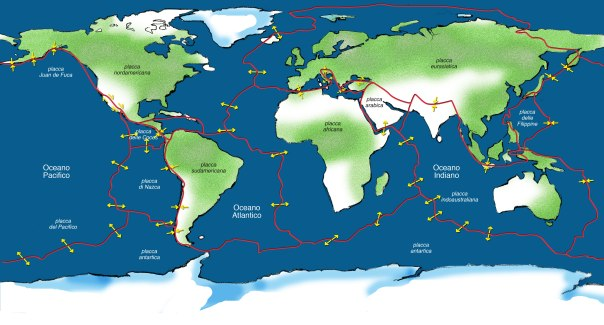
\includegraphics[width=0.835\textwidth]{images/placcheTettoniche.jpg}
   \caption{Placche tettoniche}
\end{figure}
Detto ci\`o possiamo analizzare pi\`u nel dettaglio la pericolosit\`a di una determinata zona rispetto ad un'altra. Questo discorso \`e strettamente correlato con la previsione dei terremoti.\\
La pericolosit\`a \`e quindi un'analisi della probabilit\`a che un certo scuotimento avvenga nel prossimo futuro. L'analisi pu\`o essere basata su molti fattori, ad esempio una \`e l'analisi dei \textbf{precursori}\footnote{Fenomeno anomalo che potrebbe dare un avvertimento di un terremoto imminente}, quali:
\begin{itemize}
    \item Comportamento animale;
    \item Dilatanza-diffusione;
    \item Cambiamenti in V\ped p/V\ped s;
    \item Emissioni di radon;
    \item Anomalie elettromagnetiche.
\end{itemize}
Ad oggi la validit\`a della maggioranza dei fenomeni proposti come precursori rimane indimostrata, soprattutto a causa della mancanza di osservazioni sufficientemente prolungate e sistematiche. I terremoti forti, infatti, sono eventi rari e ciascun fenomeno considerato precursore \`e caratterizzato da fluttuazioni proprie, non legate alla sismicit\`a.\\
Un altra analisi che pu\`o essere fatta per calcolare la pericolosit\`a di determinate zone, \`e l'analisi dei dati storici, che abbiamo a nostra disposizione.\\
L'analisi dei terremoti con l'obiettivo di fare previsioni, \`e oggetto di studio di migliaia di esperti, sparsi nel mondo.\\
Nel 2004 \`e stata rilasciata dall'\textbf{INGVterremoti}\footnote{Sezione dell'INGV che si occupa solo ed esclusivamente dei terremoti} la seguente mappa, che fornisce un quadro delle aree pi\`u pericolose in Italia.
\begin{figure}[H]
   \centering
   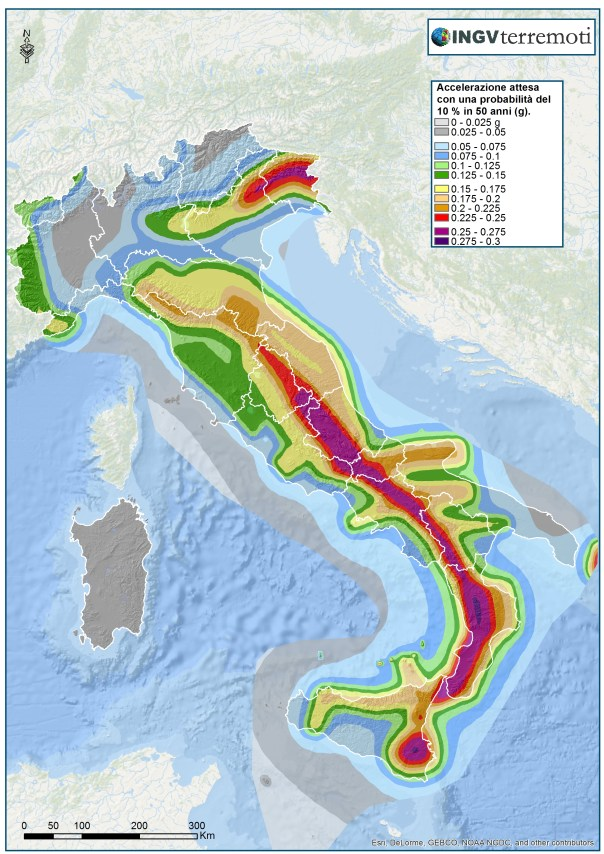
\includegraphics[width=0.5\textwidth]{images/mappaPericolosita.jpg}
   \caption{Mappa di pericolosit\`a sismica del territorio nazionale}
   \label{img:mappaPericolo}
\end{figure}
Infine l'Agenzia Spaziale Italiana ha finanziato un progetto chiamato SISMA, che utilizza tecniche di osservazione satellitari ed, in pi\`u, tiene aggiornate le previsioni a medio termine grazie a due algoritmi (CN e M8S). \cite{GiulianoFPanza}

\subsubsection{Algoritmi di previsione \textit{``M8'' e ``CN''}}

A cavallo tra gli anni '80 e '90 sono stati sviluppati due algoritmi, \textit{M8} (Keilis-Borok \& Kossobokov, 1984) e \textit{CN} (Keilis-Borok \& Rotwain, 1990) che hanno preso piede nel campo delle previsioni sismiche, sono tutt'ora utilizzati in tutto il mondo e dal Luglio 2003 anche in Italia.\\
Questi due algoritmi sono simili tra loro: utilizzano l'informazione contenuta nei cataloghi sismici, ed individuano le variazioni sismiche, che possono essere interpretate come precursori di un terremoto con magnitudo superiore ad una determinata soglia. L'analisi permette di determinare gli intervalli temporali, chiamati TIP\footnote{Times of Increased Probability (Tempi di Maggiore Probabilit\`a)}, in cui la probabilit\`a che si verifichi un terremoto con magnitudo superiore ad M0\footnote{Momento sismico. \`E utilizzato dai sismologi per misurare la quantit\`a di energia rilasciata da un terremoto}, risulta aumentata rispetto alle normali condizioni.\\
\begin{itemize}
    \item[\textbf{M8} -] Il prototipo dell'algoritmo M8 \`e stato presentato al 27\ap{o} Congresso geologico di Mosca.
L'algoritmo post-predisse il verificarsi dei terremoti di magnitudo 8.0 ed oltre in tutto il mondo, da questo deriva il nome M8.\\
Nel 1985 questo algoritmo \`e stato semplificato e riassemblato per essere applicato anche nella previsione terremoti di minore entit\`a, preservando lo schema e la definizione generale. Questa modifica \`e stata testata retroattivamente su 12 grandi terremoti verificatisi nelle regioni sismiche, principalmente nel territorio dell'URSS.\\
Durante gli anni successivi l'algoritmo M8 \`e stato testato in applicazioni per predire grandi terremoti avvenuti nel passato in altri territori. Entro il 1990, erano stati previsti in anticipo due terremoti: il terremoto di Spitak (Armenia) del 7 dicembre 1988, M = 6.9 e il terremoto di Loma Prieta (California) di ottobre 18, 1989, M = 7.1. Le previsioni furono pubblicate prima dei terremoti. \cite{algortimoM8}\\
Questo algoritmo analizza delle aree circolari, quindi i suoi rilevamenti faranno riferimento all'area nel cerchio definito inizialmente. L'algoritmo M8 scarta a priori le \textbf{scosse di assestamento}\footnote{Le scosse di assestamento sono fenomeni che si verificano dopo un terremoto di grande intensit\`a ovvero un raggruppamento di terremoti con intensit\`a minore rispetto a quello principale} rimuovendole dal catalogo preso in considerazione, in base a delle funzioni che definiscono tempo e distanza basandosi sulla grandezza del terremoto principale. Riporto di seguito la tabella che definisce queste funzioni.

\begin{figure}[H]
   \centering
   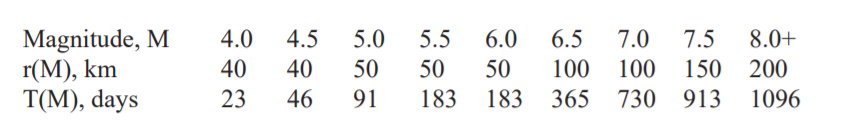
\includegraphics[width=0.850\textwidth]{images/TabellaScosseAssestamento.png}
   \caption{Tabella scosse assestamento estratta da \cite{M8Manual}}
   \label{img:tabellaScosseAssestamento}
\end{figure}

L'algoritmo decide di impostare un taglio in base alla completezza del catalogo, ovvero prendere gli eventi di una magnitudo maggiore di una certa x, questo perch\'e i dati registrati sotto quella magnitudo x sono incompleti. Una volta tolti gli eventi che si \`e deciso di scartare prende in considerazione un numero di terremoti, in base ai quali seleziona la magnitudo, ovvero mettiamo che scegliesse 20 come numero, prender\`a l'insieme di magnitudo che produce in media 20 terremoti all'anno, quindi se analizza un intervallo di 30 anni prender\`a 600 terremoti. Infine l'algoritmo calcola con delle funzioni matematiche una stima in TIP basandosi sui terremoti presi in considerazione. \cite{M8Manual}

\item[\textbf{CN} -] Un algoritmo simile all'M8 nominato precedentemente \`e il CN. Fu proposto per esaminare i precursori di sismicit\`a, dei terremoti di magnitudo $\le$ 6.4, in California e nelle regioni adiacenti come il Nevada, da cui il nome CN (California-Nevada).\\
CN \`e strutturato in modo da consentire una diagnosi dei TIP, per il verificarsi di forti terremoti.\\
L'obiettivo dell'algoritmo CN \`e quello di poter prevedere un terremoto attraverso lo studio delle attivit\`a sismiche che precedono l'avvenimento di un terremoto forte. Ci\`o \`e possibile grazie alla quantificazione degli eventi sismici, localizzati in una determinata area.\\
La quantificazione degli eventi sismici \`e ottenuta tramite un insieme di funzioni che si basano sul tempo, applicate a una sequenza di eventi avvenuti in una determinata area (escluse le scosse di assestamento). Queste funzioni quindi descrivono il livello di attivit\`a sismica, ma anche di inattivit\`a, di uno spazio-tempo, clusterizzando questi eventi.\\
Calcolate le funzioni necessarie, come ad esempio:
\begin{itemize}
    \item il livello di attivit\`a sismica;
    \item inattivit\`a sismica;
    \item variazione temporale di simicit\`a;
    \item concentrazione spaziale;
    \item clustering di terremoti.
\end{itemize}
Otteniamo il vettore P(k,t) = [p1(k,t) ... pm(k,t)] dove p(k,t) \`e una delle funzioni elencate prima.\\
Dato un tempo t e un parametro numerico r, vogliamo sapere se l'intervallo (t, t+r) appartiene a un TIP di scossa principale o di una scossa premonitrice di magnitudo M $>$ M0 nella regione k.
Questo problema \`e chiamato ``pattern recognition''. \cite{TipsCN}\\
L'allarme per il TIP \`e identificato quando il clustering \`e alto, la sismicit\`a \`e irregolare, alta e crescente (alternando intervalli di tempo di attivit\`a sismica bassa e alta). Le previsioni CN sono caratterizzate da un'incertezza temporale dell'ordine degli anni (previsioni a medio termine), poich\'e la durata dei TIP varia da pochi mesi a qualche anno e da un'incertezza spaziale di centinaia di chilometri (previsioni a medio raggio), corrispondente a un'intera singola regione monitorata. Secondo l'algoritmo, quando viene dichiarato un TIP, il forte terremoto potrebbe verificarsi in qualsiasi punto dell'area allertata, pertanto le regioni definite dovrebbero essere le pi\`u piccole possibili. \cite{algortimoCN}
\end{itemize}
Come gi\`a accennato sopra, dal Luglio del 2003 gli algoritmi CN ed M8 sono utilizzati per un collaudo sul territorio italiano. I risultati ottenuti sono i seguenti:\\
M8 ha previsto 17 dei 28 eventi di magnitudo 5.5$<$M$<$5.9 con un livello di confidenza\footnote{La definizione tecnica e completa di livello di confidenza \`e difficile da spiegare in poche righe, pertanto rimando a Wikipedia. Mi limiter\`o a fare un esempio: livello di confidenza del 99\%, presi 100 campionamenti casuali, in 99 di questi la previsione sar\`a giusta, mentre in 1 sar\`a sbagliata} superiore al 98\%.\\
CN ha previsto 12 dei 14 terremoti forti avvenuti entro le tre zone monitorate con un livello di confidenza superiore al 99\%. \cite{GiulianoFPanza}

\section{Big Data}\label{bigData}

\subsection{Cosa \`e?}
Dalla traduzione italiana abbiamo ``grandi dati'', ma io preferisco tradurlo con ``mole di dati'', questo perch\'e secondo me viene resa al meglio l'idea del concetto Big Data.\\
Big Data \`e per l'appunto una grande raccolta di dati, che nella maggior parte dei casi non si ferma nella crescita, anzi solitamente la crescita avviene in un modo molto veloce.

\subsection{A cosa serve?}\label{aCosaServono}

Per capire cosa ce ne possiamo fare di questa mole di dati prendo in considerazione un fatto accaduto nel 2009, la scoperta di un nuovo virus influenzale.\\
Questa nuova malattia fu denominata H1N1 e come molti virus si diffuse rapidamente, quindi la paura pi\`u grande era che potesse trasformarsi in pandemia. In America il CDC\footnote{Centers for Disease Control and Prevention - Centri per il Controllo e la Prevenzione delle Malattie} ordin\`o ai medici di segnalare nel pi\`u breve tempo possibile i nuovi casi di influenza. I medici fecero quanto gli fu ordinato, ma c'era un problema, che i dati erano sempre in ritardo di una o anche due settimane, questo perch\'e non tutti i pazienti segnalavano tempestivamente la malattia, in altri casi perch\`e la malattia prima di presentare i sintomi aveva un periodo di incubazione del virus che non permetteva di accorgersi di averlo contratto nell'immediato.\\
Durante l'evolversi della situazione, gli ingegneri di Google pubblicarono uno studio sulla rivista "Nature". In sostanza sostenevano di poter prevedere la diffusione dell'infulenza. Questo avveniva confrontando le ricerche digitate dagli americani nel loro motore di ricerca con i dati pubblicati dai CDC. Vennero in questo modo trovate 45 parole-chiave che presentavano una forte correlazione con i dati pubblicati dai CDC. Cos\`i a primo impatto sembra non abbiano fatto nulla di cos\`i straordinario, perch\'e producevano gli stessi risultati di previsione dei CDC, c'era per\`o una differenza sostanziale, che lo facevano in tempo reale, e non con una o due settimane di ritardo. Questo sistema messo a punto dagli ingegneri di Google si rivel\`o molto utile alle autorit\`a sanitarie per la gestione dell'epidemia.\\
Le cose che voglio prendere in considerazione di questo esempio sono le seguenti:
\begin{itemize}
    \item Gli ingegneri di Google non erano esperti in medicina, esperti in epidemie o pandemie e non erano neanche biologi o virologi;
    \item Quello che fecero gli ingegneri non fu analizzare le zone dove il virus si era sviluppato, i cosiddetti focolai;
    \item Il sistema creato prescindeva dalle ipotesi che potevano fare gli ingegneri, ad esempio vedere a cosa miravano le ricerche degli utenti.
\end{itemize}
Quindi come si evince dai punti sopra, il sistema non si basava sul ``perch\'e'' ma era comunque pi\`u efficiente nel fornire gli stessi dati pubblicati dai CDC.\\
Proprio questo \`e il concetto di Big Data, non mira a chiedersi il perch\'e avviene qualcosa, bens\`i mette insieme la mole di dati di cui si \`e a disposizione e fornisce una correlazione che in poco tempo da una risposta alla nostra domanda iniziale.\\
Noterete una certa somiglianza con la situazione in cui ci troviamo attualmente, con la nuova patologia COVID-19. Ho infatti deciso volontariamente di portare questo esempio per rispondere alla domanda posta in partenza: ``A cosa servono i Big Data?''. Attualmente Google ha messo a disposizione i Rapporti sulla Mobilit\`a della comunit\`a in formato CSV, questi saranno disponibili per un periodo di tempo limitato a condizione che i funzionari della sanit\`a pubblica ne trovino utilit\`a nel loro lavoro per fermare la diffusione del COVID-19. Chiusa questa piccola parantesi, oltre a questo esempio che ho deciso di descrivere nel dettaglio ci sono molti altri esempi interessanti dove \`e stato sfruttato il concetto di Big Data, ne cito solo un altro che ritengo importante senza entrare nel dettaglio.\\
Oren Etzioni, Professore di Informatica all'Universit\`a di Washington, che nel 2003 fece partire una start up ``Farecast'', capace di prevedere se il prezzo di un biglietto aereo sarebbe aumentato o diminuito, aveva accesso a quasi 200 miliardi di input sui prezzi dei voli.

\subsection{Big Data analytics}

L'analisi dei Big Data, come suggerisce la frase stessa, \`e un processo durante il quale si analizza la mole di dati a disposizione e si cerca una correlazione per ottenere informazioni utili al business.\\
Anche qui voglio spiegare il concetto di analisi della mole di dati portando alla luce un esempio. Amazon.com (da adesso lo chiamer\`o pi\`u semplicemente Amazon) nasce come libreria online, aveva tra i suoi dipendenti dei redattori e critici di libri, che fornivano la loro recensione e dovevano proporre nuovi titoli che Amazon aveva in vendita. Ma il fondatore e CEO di Amazon, Jeff Bezos, voleva raccomandare i libri in base ai gusti dei suoi clienti. Per questo compito decise di utilizzare i dati che aveva raccolto fino a quel momento, per\`o inizialmente approcci\`o in modo sbagliato alla sfida che si era posto, prese un piccolo campione di dati e lo analizz\`o per scoprire affinit\`a tra i suoi clienti, suggerendo cos\`i loro i libri che aveva comprato un altro cliente che risultava essere affine. Questa tecnica non ebbe un grande successo in quanto a vendite. Successivamente un programmatore che lavorava per Amazon da tempo, Greg Linden mise appunto una soluzione, questa prevedeva di correlare tra loro i prodotti, ovvero, se si era a conoscenza di quanti clienti dopo aver comprato il libro 1 compravano il libro 2, allora il libro 2 poteva essere un buon candidato a chi aveva comprato soltanto il libro 1. Anche in questo caso notiamo (vedi Sezione \ref{aCosaServono}) come non si ha a disposizione il motivo per il quale il libro 2 venisse comprato dopo il libro 1, ma si ha a disposizione comunque l'informazione, e questa informazione economicamente parlando risult\`o essere molto pi\`u importante di scovare il motivo che mette in correlazione il libro 1 con il libro 2. Infatti il computer che analizzava la mole di dati non sapeva il perch\'e un cliente che aveva comprato un libro di "Robert B. Cialdini" volesse poi comprare un libro di "Kevin Mitnick", ma sapeva soltanto che era cos\`i, quindi Amazon cominci\`o a consigliare i prodotti ai suoi clienti in modo molto coerente e trov\`o un riscontro positivo immediato nelle vendite e nel fatturato dell'azienda.\\
Questo esempio ci fa capire quindi che pi\`u \`e grande la mole di dati da analizzare e pi\`u \`e alta la probabilit\`a che il nostro algoritmo che analizza i dati far\`a previsioni attendibili, quindi possiamo affermare che \`e pi\`u importante avere a disposizione tanti dati piuttosto che meno dati pi\`u qualitativi. \cite{bigData}

\section{Disuguaglianza di Chebyshev}\label{disuguaglianzaChebyshev}
Usando la media $\mu$ e la varianza $\sigma^{2}$ della variabile casuale X si pu\`o ricavare un ``Tail Bound''\footnote{Per una variabile casuale X le ``Tails'' di X sono le parti della funzione di densit\`a discreta che sono lontane dalla sua media, quindi un ``Tail Bound'' \`e un limite a queste ``Tails''} significativamente pi\`u forte noto come Disuguaglianza di Chebyshev.

\begin{theorem}[Chebyshev theorem]
\label{ChebyshevThm}
    $\forall a > 0$\\
    $Pr(\mid X - \mu \mid \ge a) \le \dfrac{\sigma^{2}}{a^{2}}$ 
\end{theorem}

Dal Teorema \ref{ChebyshevThm} ponendo a = $\lambda\sigma$ dove:\\
$\lambda$ = numero reale positivo (che posto a 2 permette di affermare che la probabilit\`a sia sempre maggiore del 75\%)\\
$\sigma$ = deviazione standard\\
otteniamo:

\begin{equation}
    Pr(\mid X - \mu \mid \ge \lambda\sigma) \le \dfrac{1}{\lambda^{2}}
\end{equation}

Da cui svolgendo il modulo:

\begin{equation}
    Pr(\mu - \lambda\sigma \le X \le \mu + \lambda\sigma) \le \dfrac{1}{\lambda^{2}}
\end{equation}

Che equivale a scrivere:

\begin{equation}\label{chebyshev}
    Pr(\mu - \lambda\sigma \le X \le \mu + \lambda\sigma) \ge 1 - \dfrac{1}{\lambda^{2}}
\end{equation}

Quindi ho ottenuto la Formula \ref{chebyshev} che mi dice che la probabilit\`a che la variabile casuale X assuma valori compresi nell'intervallo definito tra parentesi sar\`a almeno 1 - $\dfrac{1}{\lambda^{2}}$. \cite{probAndComputing}